\documentclass{article}
\usepackage[dvipsnames]{xcolor}
\usepackage[paperwidth=20cm, paperheight=8cm, margin = 0cm, top=0.5cm]{geometry}

\usepackage{pgf}
\usepackage{tikz}
\usetikzlibrary{arrows,automata}
\usetikzlibrary{positioning}

\tikzstyle{source}  = [draw,circle,fill=black,thick,inner sep=0mm,minimum size=2mm]
\tikzstyle{box}  = [draw,rectangle,thick,inner sep=2mm,minimum width=8mm, minimum height=8mm]

\begin{document}
\begin{center}
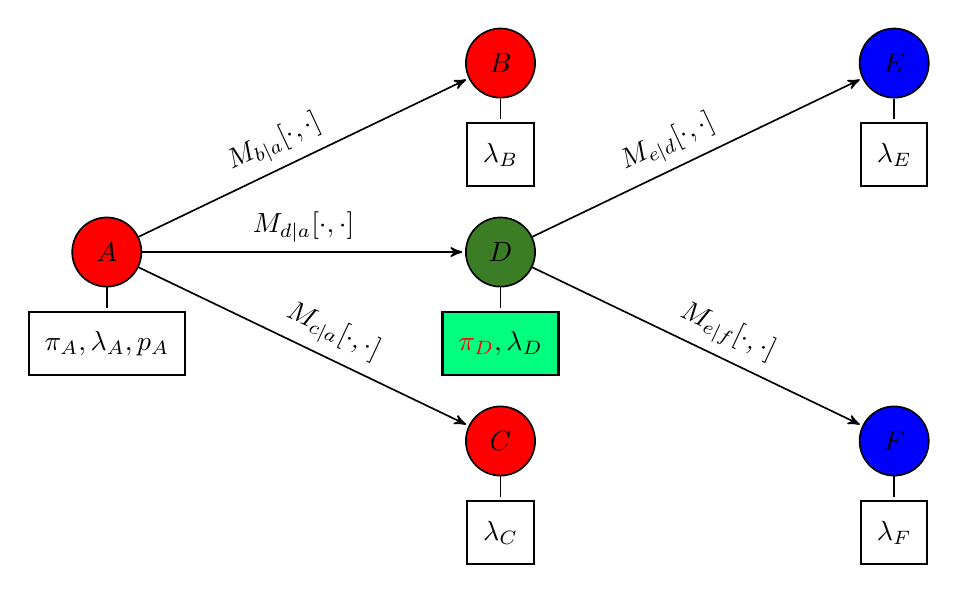
\begin{tikzpicture}[->,>=stealth',shorten >=1pt,auto,node distance=5cm,semithick]
                    
\node[state, fill=red]  (X1)               {$A$}; 
\node[state, fill=OliveGreen] (X2) [right of=X1] {$D$};
\node[state, fill=red] (X3) [above=1.5cm of X2]        {$B$};                   
\node[state, fill=red] (X4) [below=1.5cm of X2]        {$C$};                   
\node (X5) [right of=X2] {};
\node[state, fill=blue] (X6) [right of=X3] {$E$};                   
\node[state, fill=blue] (X7) [right of=X4] {$F$}; 

\node[box][below=0.3cm of X1](P1){$\pi_A,\lambda_A,p_A$};                  
\node[box][below=0.3cm of X3](P3){$\lambda_B$};                  
\node[box][below=0.3cm of X4](P4){$\lambda_C$};                  
\node[box, fill=SpringGreen][below=0.3cm of X2](P2){$\textcolor{red}{\pi_D},\lambda_D$};                  
\node[box][below=0.3cm of X6](P6){$\lambda_E$};                  
\node[box][below=0.3cm of X7](P7){$\lambda_F$};                  

\path
	(X1) edge node {$M_{d|a}[\cdot,\cdot]$} (X2)
	(X1) edge node[rotate=25, xshift=0.5cm] {$M_{b|a}[\cdot,\cdot]$} (X3)
	(X1) edge node[rotate=-25, xshift=-0.5cm] {$M_{c|a}[\cdot,\cdot]$} (X4)
	(X2) edge node[rotate=25, xshift=0.5cm] {$M_{e|d}[\cdot,\cdot]$} (X6)
	(X2) edge node[rotate=-25, xshift=-0.5cm] {$M_{e|f}[\cdot,\cdot]$} (X7);

\path
	(X1) edge[-] (P1)
	(X3) edge[-] (P3)
	(X4) edge[-] (P4)
	
	(X2) edge[-] (P2)
	(X6) edge[-] (P6)
	(X7) edge[-] (P7);

\end{tikzpicture}
\end{center}

\end{document}
